\documentclass[12pt]{article}
%\usepackage{fullpage}
\usepackage{epic}
\usepackage{eepic}
\usepackage{paralist}
\usepackage{graphicx}
\usepackage{algorithm,algorithmic}
\usepackage{tikz}
\usepackage{xcolor,colortbl}
\usepackage{amsmath, amssymb}

%%%%%%%%%%%%%%%%%%%%%%%%%%%%%%%%%%%%%%%%%%%%%%%%%%%%%%%%%%%%%%%%
% This is FULLPAGE.STY by H.Partl, Version 2 as of 15 Dec 1988.
% Document Style Option to fill the paper just like Plain TeX.

\typeout{Style Option FULLPAGE Version 2 as of 15 Dec 1988}

\topmargin 0pt
\advance \topmargin by -\headheight
\advance \topmargin by -\headsep

\textheight 8.9in

\oddsidemargin 0pt
\evensidemargin \oddsidemargin
\marginparwidth 0.5in

\textwidth 6.5in
%%%%%%%%%%%%%%%%%%%%%%%%%%%%%%%%%%%%%%%%%%%%%%%%%%%%%%%%%%%%%%%%

\pagestyle{empty}
\setlength{\oddsidemargin}{0in}
\setlength{\topmargin}{-0.8in}
\setlength{\textwidth}{6.8in}
\setlength{\textheight}{9.5in}

\setcounter{secnumdepth}{0}

\setlength{\parindent}{0in}
\addtolength{\parskip}{0.2cm}
\setlength{\fboxrule}{.5mm}\setlength{\fboxsep}{1.2mm}
\newlength{\boxlength}\setlength{\boxlength}{\textwidth}
\addtolength{\boxlength}{-4mm}

\newcommand{\algosolutionbox}[2]{
  \begin{center}
    \framebox{\parbox{\boxlength}{
        \textbf{CS 5722, Fall 2014} \hfill \textbf{#1}\\
        #2
      }}
  \end{center}}

\begin{document}

\algosolutionbox{Homework 13}{
  % TODO: fill in your own name, netID, and collaborators
  Group: Michael Jalkio, Kevin Li, Daniel Sperling\\
  NetIDs: mrj77, kyl27, dhs252
}

\section{1a}
The equation is:
\begin{align*}
f(x) & = x + ((x + (((x + (cos(x-x) - (x-x))) * x) * x))*x)\\
& = x + ((x + (((x + (cos(0) - 0)) * x) * x))*x)\\
& = x + ((x + (((x + 1) * x) * x))*x)\\
& = x + ((x + ((x^2 + x) * x))*x)\\
& =  x + ((x + x^3 + x^2)*x)\\
& = x + (x^2 + x^4 + x^3)\\
& = x^4 + x^3 + x^2 + x
\end{align*}

\subsection{b}
The only unnecessary term is $(-XX)$ that is subtracted from the cosine term.  The subtree $(-(COS(-XX))(-XX))$ could simply be $(COS(-XX))$.

\section{2a}
Objective: $X^2/2 + 2X + 2$\\
Terminal Set: $X$
Function Set: addition, subtraction, multiplication, and protected division.
Parameters: Population size 1000, max generations 151

\subsection{b}
The best fitness at generation zero was 6.85 for a tree with 23 nodes:\\
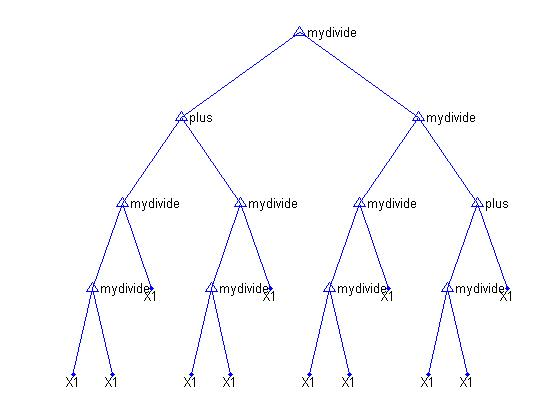
\includegraphics[scale=0.5]{gen_0}

\subsection{c}
An intermediate solution was found at fitness 5.85 with 9 nodes, representing 2X + 2. This solution was actually found quickly, in generation 1, and lasted for many generations as the best. It is significantly simpler than the first generation, and comes very close to approximating the real solution (has two terms correct, 2X + 2). It is notably worse than the best solution, though, as it does not have any attempt at multiplication, which would give the remaining term:\\
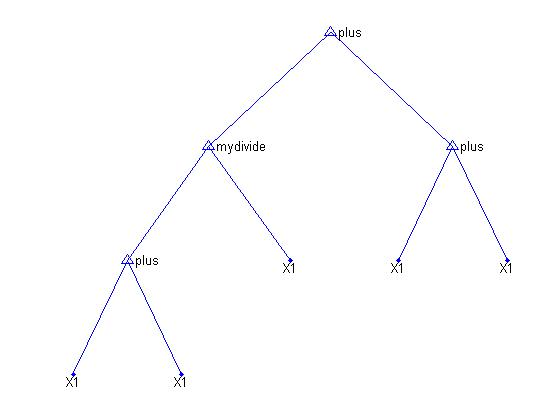
\includegraphics[scale=0.5]{intermediate}

\subsection{d}
The best-of-run individual had fitness 4.1462 and had 23 nodes. It represents 2X + 2:\\
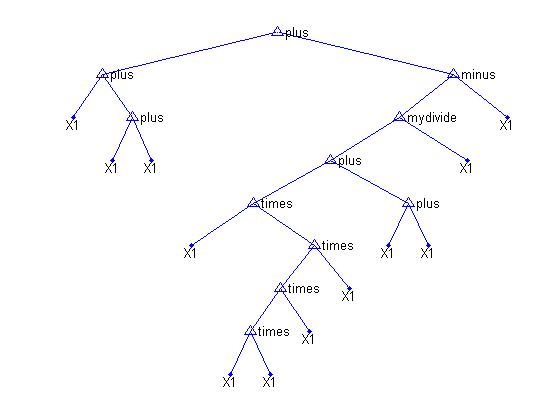
\includegraphics[scale=0.5]{best}

\subsection{e}
No, this was an approximation.

\subsection{f}
After many runs, the code continues to return to a fitness no better than 4.1462 as the best after 151 generations.

\section{3a}
The summary of the Santa Fe policy from lecture is:
\begin{enumerate}
  \item Move ahead if there is food
  \item If no food turn left and move ahead if food
  \item Otherwise turn right twice and move ahead if food
  \item Otherwise turn left and move even though there is no food
\end{enumerate}
This is not optimal for the Los Altos trail.  The main reason is that it needs the ant to be directly next to a piece of food for it to change its direction.  This does not happen at locations 116 an 136 on the Los Altos trail.  At these locations the Santa Fe policy would cause the ant to continue moving downward, it would never turn to continue to follow the path.

\subsection{b}
% Honestly I'm not quite sure why you would use any different functions or terminals...
% Maybe you could add more ProgNm functions?  Not sure why that would be helpful.

\section{4}
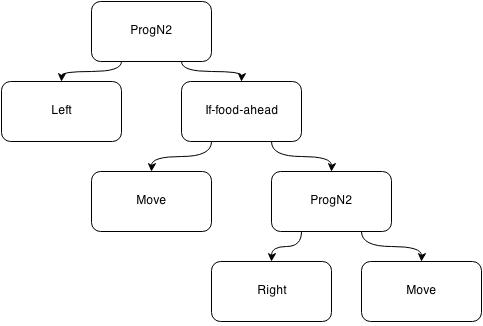
\includegraphics{problem4}

\section{5a}
1 piece of food is eaten, the one at the start.  The 10 steps taken are:
\begin{center}
[Move, Move, Move, Move, Move, Move, Move, Move, Move, Nothing]
\end{center}

\subsection{b}
3 pieces of food are eaten.  The 10 steps taken are:
\begin{center}
[Right, Left, Move, Right, Move, Move, Right, Left, Move, Right]
\end{center}

\end{document}